\chapter{Statistical Analysis and Graph}

This module is responsible for creating the statistics and Graphs for visulalization and analysis. This 
module proves to be very important for debugging. Currently only two components are implemented but more
can be implemented in future as per the need.

\section{Log generatotion}
This component generates all the log in the system. There are two sets of log. One corresponding to each train that gives 
info about the status of the train at different times during the simulation. Another generates log corresponding 
to the status of the network, how many trains are there in the network and wether the network is in deadlock or not. All 
logs are generated and put in the folder \textbf{Log}.

\section{Graphs for visulalization}
This component creates graph for visualization, while the simulation is running. Amount of detail 
we want in the graph can be controlled using different arguments. Note that this component slows down the simulation,
so when the learning algorithm is running we can turn off this component.

\subsection{Details of the image} 
Each station is represented by node and each track is represented by edge
connecting these nodes. There can be more than one railway line on station or track, so the width of the 
nodes or the edges is directly propotional to the number of railway lines on that resource. How many lines 
are free on a given resource, that is encoded using the labels (on nodes and edges) and light green color. 
Each train running in the network is color coded. If more than 8 trains are running in the network, then all the trains
will have the same color (then image just shows the resource level information about each resource in the network).
We can control the amount of detail in the network by passing different arguments. For more details, look into the 
code repository. 


\begin{figure}[h]
    \centering
    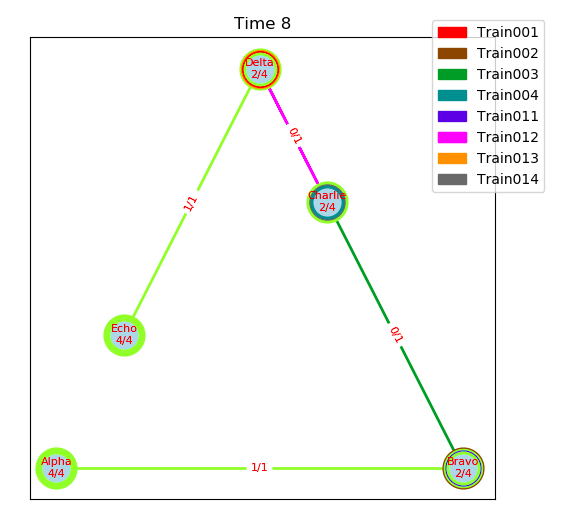
\includegraphics[width=0.6\textwidth]{graph}
    \caption{ Network with trains color coded.  }
    \label{image-myimage5}
\end{figure}

\begin{figure}[h]
    \centering
    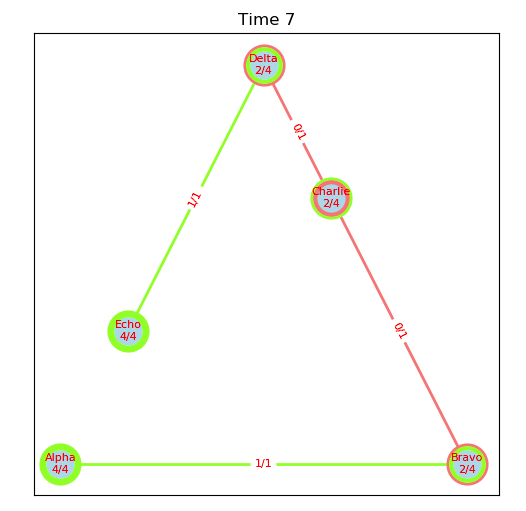
\includegraphics[width=0.6\textwidth]{graph2}
    \caption{ Network showing just what all resources are free.  }
    \label{image-myimage6}
\end{figure}